\chapter{Combinatoria delle parole}

\subsubsection{Lemma di Levi}

Siano $u, v, x, y \in A^{*}$ e supponiamo che $u v=x y .$ Se $|u| \geq|x|$, esiste $t \in A^{*}$ tale che $u=x t$ e $y=t v .$ Se $|u|<|x|$, esiste $t \in A^{+}$ tale che $x=u t $e$ v=ty$.

\begin{figure}[hbpt!]
    \centering
    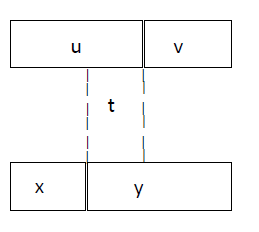
\includegraphics[width=4cm]{./Images/9.1.png}
\end{figure}
\FloatBarrier

\subsubsection{Primo Teorema di Lyndon-Schutzenberger}
Siano $x, y, z \in A^{+} .$Allora $x y=y z$ se e solo se esistono $u \in A^{+}$,
$v \in A^{*}$ e un intero $e \geq 0$ tali che $x=uv $ e $ z=v u $ e 
$y=(u v)^{e} u=u(v u)^{e} .$

\subsubsection{Secondo Teorema di Lyndon-Schutzenberger}

Siano $x, y, z \in A^{+}$. Le seguenti tre condizioni sono equivalenti.
\begin{enumerate}
    \item $x y=y x$.
    \item Esistono $z \in A^{+}$e interi $h, k>0$ tali che $x=z^{h}$ e $y=z^{k}$.
    \item Esistono interi $i, j>0$ tali che $x^{i}=y^{j}$.
\end{enumerate}


\subsubsection{Parole}

Una parola $w$ è primitiva se $w=v^{n}$ implica $n=1$. Nota che la parola vuota non è primitiva.

\vspace{5mm}

\textbf{Proposizione}

Ogni parola non vuota è potenza di un'unica parola primitiva.

\vspace{5mm}

Due parole $x, y$ sono coniugate se esistono parole $u, v$ tali che $x=u v, y=v u .$ La relazione di coniugazione è una relazione di equivalenza.

Una classe di coniugazione è una classe di questa relazione di equivalenza.

Una classe di coniugazione è spesso chiamata \textit{necklace}.

\vspace{5mm}

Se $w$ è una parola primitiva, tutte le sue coniugate sono primitive. 
Un necklace è primitivo se è la classe di coniugazione di una parola primitiva.

\vspace{5mm}

Una parola primitiva di lunghezza $n$ ha $n$ distinte coniugate.

Infatti assumiamo $r s=s r$ con $r, s$ non vuote.

Per il secondo teorema di Lyndon-Schutzenberger esiste una parola $x$ tale che $r=x^{i}, s=x^{j}$ e $r s=x^{i+j}$ non è primitiva.

\subsubsection{I sei necklace primitivi di lunghezza 5 sull'alfabeto \{a,b\}}

\begin{figure}[hbpt!]
    \centering
    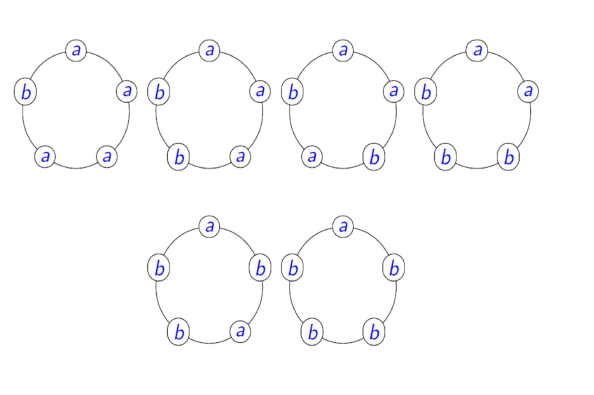
\includegraphics[width=6cm]{./Images/9.2.png}
\end{figure}
\FloatBarrier

\subsubsection{Ordine lessicografico}

Sia $A=\left\{a_{0}, \ldots, a_{k}\right\}$ un alfabeto e sia $a_{0}<a_{1}<\ldots<a_{k}$ un ordinamento degli elementi di $A$. Siano $x, y \in A^{*}$.

Diremo che $x<y$ rispetto all'ordine lessicografico se $x$ e $y$ verificano una delle condizioni seguenti:
\begin{enumerate}
    \item $y=x z \operatorname{con} z \in A^{+}$, cioè $x$ è un prefisso di y e x $\neq$ y.
    \item $x=z a x^{\prime}, y=z b y^{\prime}, \operatorname{con} z, x^{\prime}, y^{\prime} \in A^{*}, a, b \in A e a<b$.
\end{enumerate}
Le parole in un dizionario sono ordinate in base all'ordine lessicografico.
\textbf{Esempio.} Supponiamo $a<b<\ldots<z$.

\vspace{5mm}

\begin{center}
    latte $<$ latteria, castagna $<$ castello.
\end{center}

\vspace{5mm}

Siano $x, y \in A^{*}$. Valgono le seguenti proprietà.
\begin{enumerate}
    \item $x<y$ se e solo se $z x<z y$, per ogni $z \in A^{*}$.
    \item If $x<y e x$ non è prefisso di $y$, allora $x u<y v$ per ogni $u, v \in A^{*} .$
\end{enumerate}

\subsubsection{Parole di Lyndon}

Una parola di Lyndon è una parola primitiva che è minore di tutte le sue coniugate rispetto all'ordine lessicografico. Denotiamo con $L$ l'insieme delle parole di Lyndon.

Le "prime" parole di Lyndon su $\{a, b\}$, con $a<b$.
$$
\begin{gathered}
a, b \\
a b \\
a a b, a b b \\
a a a b, a a b b, a b b b \\
aaaab, aa a b b, a abab, a abbb, ababb, abbbb 
\end{gathered}
$$

Una parola è una parola di Lyndon se e solo se è minore di ogni suo suffisso proprio diverso dalla parola vuota.
\begin{itemize}
    \item \textbf{Sufficienza:} sia $w=u v$ con $u, v$ non vuote. Poiché $w<v$, risulta $w<v u$. Inoltre $w$ è primitiva altrimenti $w=z^{n}$ con $n>1$ e quindi $z<w<z$, una contraddizione.
    \item \textbf{Necessità:} sia $w \in L$ e sia $w=u v$ con $u, v$ non vuote. Assumiamo prima che $w=v t$. Poiché $w$ è una parola di Lyndon, $w<t v$. Ma $u v<t v$ implica $u<t$ e quindi $v u<v t$, una contraddizione.
\end{itemize}
Quindi $v$ non è un prefisso di $w .$ Ma $v<u v$ implicherebbe allora $v u<u v$, una contraddizione. Concludiamo che $u v<v .$

\vspace{5mm}

Se $\ell, m \in L \operatorname{con} \ell<m$, allora $\ell m$ è una parola di Lyndon.

\vspace{5mm}


\textbf{Prova (cenni).}

Mostriamo prima che $\ell m<m .$ Se $\ell$ è un prefisso di $m$, allora $m=\ell m^{\prime}$. Quindi $m<m^{\prime}$ implica $\ell m<\ell m^{\prime}=m$. Altrimenti $\ell$ non è un prefisso di $m$ e allora $\ell<m$ implica $\ell m<m$.

Sia $v$ un suffisso proprio non vuoto di $\ell m$. Se $v$ è un suffisso di $m$, allora $m<v$ e allora $\ell m<m<v$. Altrimenti, abbiamo $v=v^{\prime} m$. Quindi $\ell<v^{\prime}$ e allora $\ell m<v^{\prime} m=v$.

\subsubsection{Il teorema della fattorizzazione}

\textbf{Teorema (Lyndon)}

Ogni parola si fattorizza in modo unico come un prodotto di parole di Lyndon in cui ogni fattore è maggiore o uguale al successivo (nonincreasing product).

Quindi ogni parola $w$ può essere scritta in modo unico
$$
w=\ell_{1} \cdots \ell_{m}
$$
$\operatorname{con} \ell_{1}, \ldots, \ell_{m} \in L \in \ell_{1} \geq \ldots \geq \ell_{m}$

\vspace{5mm}

\begin{itemize}
    \item \textbf{Esistenza:} Poiché le lettere sono in $L$, ogni parola ha una fattorizzazione in parole di Lyndon.
\end{itemize}

Consideriamo una fattorizzazione $w=\ell_{1} \cdots \ell_{m}$ in parole di Lyndon e con $m$ minimale. Se $\ell_{i}<\ell_{i+1}$ per qualche $i$, allora $w=\ell_{1} \cdots \ell_{i-1}\left(\ell_{i} \ell_{i+1}\right) \cdots \ell_{m}$ è una fattorizzazione in parole di Lyndon poiché $\ell_{i} \ell_{i+1} \in L$.

\begin{itemize}
    \item Unicità: Assumiamo che $\ell_{1} \cdots \ell_{m}=\ell_{1}^{\prime} \cdots \ell_{m^{\prime}}^{\prime}$ con $\ell_{i}, \ell_{i}^{\prime} \in L$, $\ell_{1} \geq \ldots \geq \ell_{m}$ e $\ell_{1}^{\prime} \geq \ldots \geq \ell_{m^{\prime}}^{\prime}$. Assumiamo che $\ell_{1}$ è più lunga di $\ell_{1}^{\prime}$. Quindi $\ell_{1}=\ell_{1}^{\prime} \cdots \ell_{i}^{\prime} u$ con $u$ prefisso non vuoto di $\ell_{i+1}^{\prime}$. Allora $\ell_{1}<u \leq \ell_{i+1}^{\prime} \leq \ell_{1}^{\prime}<\ell_{1}$, una contraddizione.
\end{itemize}

\subsubsection{Sesquipotenze di parole di Lyndon}

Sia $P$ l'insieme di tutte le parole che sono diverse dalla parola vuota e che sono prefissi di qualche parola di Lyndon.

Una sesquipotenza di una parola $x$ è una parola $w=x^{n} p$ con $n \geq 1$ e con $p$ prefisso proprio di $x$.


\textbf{Proposizione}

L'insieme $P$ è l'insieme delle sesquipotenze delle parole di Lyndon diverse dalla lettera massimale.

\vspace{5mm}

La prova usa il lemma seguente.

\vspace{5mm}


\textbf{Lemma}

Per ogni parola $p$ e a $\in A$ tali che pa è un prefisso di una potenza di una parola di Lyndon, e per ogni lettera $b>a, p b$ è una parola di Lyndon.

\vspace{5mm}

Sia $x \in L$, dove $x$ non è una potenza della lettera massimale. Poniamo $x=p a q$ con a una lettera non massimale. Allora ogni prefisso di $x^{n}$ è un prefisso di $w=x^{n} p b$ con $b>a$ e $w$ è in $L$.

Viceversa sia $w$ un prefisso di $x \in L$ diverso dalla parola vuota. Usiamo l'induzione su $|w|$. Se $|w|=1$, allora $w \in L$. Assumiamo $|w|>1$. Poniamo $w=v a$ con $a \in A$. Per ipotesi induttiva, $v=y^{n} p$ con $y \in L, n \geq 1$ e con $p$ prefisso proprio di $y$. Poniamo $y=p b u \operatorname{con} b \in A$. Poiché $w$ è un prefisso di una parola di Lyndon, abbiamo $p b \leq p a($ da $w s=x<p a s)$ e allora $b \leq a$. Se $a=b$, allora $w$ è una sesquipotenza di $y .$ Se $b<a, w \in L$ per il lemma precedente.





\let\cleardoublepage\clearpage

